% Select one class
%\documentclass{pucthesis}		% For DVI
\documentclass[pdftex]{pucthesis}	% For pdfLaTeX
%\documentclass[spanish]{pucthesis}		% For DVI, in spanish
%\documentclass[pdftex,spanish]{pucthesis}	% For pdfLaTeX, in spanish

%%%%%%%%%%%%%%%%%%%%%%%%%%
%      Nota: si usas español, algunos nombres      %
%      debes cambiarlos manualmente en este     %
%        documento. En teoría, nunca deberías       %
%           modificar el archivo pucthesis.cls              %
%%%%%%%%%%%%%%%%%%%%%%%%%%

%%%%%%%%%
%   Packages	 %
%%%%%%%%%

% Floats
\usepackage{graphicx}
\usepackage{float}
\floatstyle{boxed}
\restylefloat{figure}
\usepackage{subfigure}
\usepackage{color}

% Math packages
\usepackage{amsmath}
\usepackage{amsfonts}
\usepackage{amssymb}

% Closest font to Times New Roman
\usepackage{times}

% To make pretty tables
\usepackage{booktabs}
\usepackage{multirow}

% To avoid underfull errors in the bibliography
\usepackage{etoolbox}
\apptocmd{\sloppy}{\hbadness 10000\relax}{}{}

% To make cites and references
\usepackage[hidelinks,pdfusetitle,pdfdisplaydoctitle]{hyperref}
\usepackage[notocbib]{apacite} 
\usepackage{doi}
\renewcommand{\doitext}{}

%--------- NEW ENVIRONMENTS --------- You are free to remove or use it
\newtheorem{definition}{\bf Definition}[chapter]
\newtheorem{property}{Property}[chapter]
\newtheorem{claim}{Claim}[chapter]
\newtheorem{lemma}{\bf Lemma}[chapter]
\newtheorem{proposition}{Proposition}[chapter]
\newtheorem{theorem}{\noindent \bf Theorem}[chapter]
\newtheorem{corollary}{\bf Corollary}[chapter]
\newtheorem{pf}{Proof}[chapter]
\newtheorem{example}{\bf Example}[chapter]
\newtheorem{remark}{Remark}[chapter]

<<<<<<< HEAD
\makeatletter
  \setlength{\beftitle}{105\p@\@plus24\p@}
  \setlength{\afttitle}{65\p@}
\makeatother
=======
% En caso de que el título sea muy largo, se puede ajustar el espacio
% antes y después de este en las dos primeras páginas para que quede centrado.

%\makeatletter
%  \setlength{\beftitle}{105\p@\@plus24\p@}
%  \setlength{\afttitle}{65\p@}
%\makeatother
>>>>>>> origin/master

\begin{document}

\mdate{Month Day, Year}         % date manuscript changed
\version{1}                                     % manuscript version #

\title[(LONG THESIS TITLE)]
   {\bf (LONG THESIS TITLE)}       
\author[Author's Name]{Author's name}

\address{Escuela de Ingenier\'ia\\
                   Pontificia Universidad Cat\'olica de Chile\\ 
                   Vicu\~na Mackenna 4860\\
                  Santiago, Chile\\
                  {\it Tel.\/} : 56 (2) 354-2000}
\email{username@uc.cl}

\facultyto    {the School of Engineering}
%\department   {}
\faculty                             {Faculty of Engineering}
\degree                  {Master of Science in Engineering}  %   {Mag\'ister en Ciencias de la Ingenier\'ia}  %        
                                 % or {Doctor in Engineering Sciences}    % {Doctor en Ciencias de la Ingenier\'ia}
\advisor                            {Professor's name}
\committeememberA {Member A}
\guestmemberA            {Member B}
\ogrsmember                 {Member C}
\subject                            {Structural Engineering}
\date                                 {Month Year}
\copyrightname             {Author's name}
\copyrightyear               {MMXV}
\dedication                      {Gratefully to my parents and siblings}

%%%%%%%%%%%%%%%%%%%%
%       PRELIMINARIES                              %
%----------------------------------------------------%
%      page i & ii: cover page                   %
%      page iii: dedication                         %
%%%%%%%%%%%%%%%%%%%%

\NoChapterPageNumber
\pagenumbering{roman}
\maketitle

%%%%%%%%%%%%%%%%%%%%
%   EXTRA PAGES                                     %
%----------------------------------------------------%
%      page --: not used                             %
%%%%%%%%%%%%%%%%%%%%

%\newpage
%\thispagestyle{empty}

%----------------------------------------------------------------------%

%%%%%%%%%%%%%%%%%%%%%%%%%
%      page v: ACKNOWLEDGEMENTS                   %
%%%%%%%%%%%%%%%%%%%%%%%%%

\phantomsection \label{acknowledgements} % Comment if hyperref is unused
\chapter*{ACKNOWLEDGEMENTS}           
Write in a sober style your acknowledgements to those persons that contributed to the development and preparation of your thesis.



\cleardoublepage

%----------------------------------------------------------------------%

%%%%%%%%%%%%%%%%%%
%          page v & up ---                      %
%            Table of contents              %
%            List of figures                     %
%            List of tables                      %
%%%%%%%%%%%%%%%%%%

\pdfbookmark{\contentsname}{toc}
\tableofcontents
\phantomsection \label{listoffigures}
\listoffigures
\phantomsection \label{listoftables}
\listoftables
\cleardoublepage

%----------------------------------------------------------------------%

%%%%%%%%%%%%%%%%%%%%%%%%
%      page x & xi: ABSTRACT - RESUMEN        %
%%%%%%%%%%%%%%%%%%%%%%%%

\phantomsection \label{abstract}
\chapter*{ABSTRACT}
The abstract must contain between 100 and 300 words.  The abstract must be written in English and Spanish.  In the case of doctoral theses, the layout of the abstract page is different, so please check the template provided by the OGRS. \

\vfill
\noindent {\bf Keywords}:  thesis template, document writing, {\bf (Write here the keywords relevant and strictly related to the topic of the thesis)}.

\cleardoublepage

\phantomsection \label{resumen}
\chapter*{RESUMEN}
El resumen debe contener entre 100 y 300 palabras. El resumen debe ser escrito en ingl\'es y espa\~nol.  En el caso de tesis de doctorado, el formato de la p\'agina del resumen es distinta, por favor verifique la plantilla entregada por la Direcci\'on de Postrgrado.\

\vfill
\noindent {\bf Palabras Claves}: plantilla de tesis, escritura de documentos, {\bf (Colocar aqu\'i las palabras claves relevantes y estr\'ictamente relacionadas al tema de la tesis)}.

\cleardoublepage

%%%%%%%%%%%%%
%   TEXT  OF THESIS     %
%%%%%%%%%%%%%

\pagenumbering{arabic}

\chapter[INTRODUCTION]{Introduction}
These class and template were produced based on the following idea: do not worry about the margins, focus on your calculations.

In Chapter \ref{ch1} we show how to write Sections, Sub Sections and Sub sub Sections. In Chapter \ref{ch2} we put some figures and tables.

Good luck with your thesis.

\chapter[CHAPTER 1]{Chapter 1} \label{ch1}
\section{First Section \label{sec:sec1}}
Lorem ipsum ad his scripta blandit partiendo, eum fastidii accumsan euripidis in, eum liber hendrerit an. Qui ut wisi vocibus suscipiantur, quo dicit ridens inciderint id. Quo mundi lobortis reformidans eu, legimus senserit definiebas an eos. Eu sit tincidunt incorrupte definitionem, vis mutat affert percipit cu, eirmod consectetuer signiferumque eu per. In usu latine equidem dolores. Quo no falli viris intellegam, ut fugit veritus placerat per.

Ius id vidit volumus mandamus, vide veritus democritum te nec, ei eos debet libris consulatu. No mei ferri graeco dicunt, ad cum veri accommodare. Sed at malis omnesque delicata, usu et iusto zzril meliore. Dicunt maiorum eloquentiam cum cu, sit summo dolor essent te. Ne quodsi nusquam legendos has, ea dicit voluptua eloquentiam pro, ad sit quas qualisque. Eos vocibus deserunt quaestio ei.

Blandit incorrupte quaerendum in quo, nibh impedit id vis, vel no nullam semper audiam. Ei populo graeci consulatu mei, has ea stet modus phaedrum. Inani oblique ne has, duo et veritus detraxit. Tota ludus oratio ea mel, offendit persequeris ei vim. Eos dicat oratio partem ut, id cum ignota senserit intellegat. Sit inani ubique graecis ad, quando graecis liberavisse et cum, dicit option eruditi at duo. Homero salutatus suscipiantur eum id, tamquam voluptaria expetendis ad sed, nobis feugiat similique usu ex.

\subsection{First SubSection \label{sec:sub1}}
Eum hinc argumentum te, no sit percipit adversarium, ne qui feugiat persecuti. Odio omnes scripserit ad est, ut vidit lorem maiestatis his, putent mandamus gloriatur ne pro. Oratio iriure rationibus ne his, ad est corrumpit splendide. Ad duo appareat moderatius, ei falli tollit denique eos. Dicant evertitur mei in, ne his deserunt perpetua sententiae, ea sea omnes similique vituperatoribus. Ex mel errem intellegebat comprehensam, vel ad tantas antiopam delicatissimi, tota ferri affert eu nec. Legere expetenda pertinacia ne pro, et pro impetus persius assueverit.

Ea mei nullam facete, omnis oratio offendit ius cu. Doming takimata repudiandae usu an, mei dicant takimata id, pri eleifend inimicus euripidis at. His vero singulis ea, quem euripidis abhorreant mei ut, et populo iriure vix. Usu ludus affert voluptaria ei, vix ea error definitiones, movet fastidii signiferumque in qui.

Vis prodesset adolescens adipiscing te, usu mazim perfecto recteque at, assum putant erroribus mea in. Vel facete imperdiet id, cum an libris luptatum perfecto, vel fabellas inciderint ut. Veri facete debitis ea vis, ut eos oratio erroribus. Sint facete perfecto no vel, vim id omnium insolens. Vel dolores perfecto pertinacia ut, te mel meis ullum dicam, eos assum facilis corpora in.

Mea te unum viderer dolores, nostrum detracto nec in, vis no partem definiebas constituam. Dicant utinam philosophia has cu, hendrerit prodesset at nam, eos an bonorum dissentiet. Has ad placerat intellegam consectetuer, no adipisci mandamus senserit pro, torquatos similique percipitur est ex. Pro ex putant deleniti repudiare, vel an aperiam sensibus suavitate. Ad vel epicurei convenire, ea soluta aliquid deserunt ius, pri in errem putant feugiat.

\subsection{Second SubSection \label{sec:sub2}}
Sed iusto nihil populo an, ex pro novum homero cotidieque. Te utamur civibus eleifend qui, nam ei brute doming concludaturque, modo aliquam facilisi nec no. Vidisse maiestatis constituam eu his, esse pertinacia intellegam ius cu. Eos ei odio veniam, eu sumo altera adipisci eam, mea audiam prodesset persequeris ea. Ad vitae dictas vituperata sed, eum posse labore postulant id. Te eligendi principes dignissim sit, te vel dicant officiis repudiandae.

Id vel sensibus honestatis omittantur, vel cu nobis commune patrioque. In accusata definiebas qui, id tale malorum dolorem sed, solum clita phaedrum ne his. Eos mutat ullum forensibus ex, wisi perfecto urbanitas cu eam, no vis dicunt impetus. Assum novum in pri, vix an suavitate moderatius, id has reformidans referrentur. Elit inciderint omittantur duo ut, dicit democritum signiferumque eu est, ad suscipit delectus mandamus duo. An harum equidem maiestatis nec.

\subsubsection{First sub sub section \label{sec:subsub1}}
At has veri feugait placerat, in semper offendit praesent his. Omnium impetus facilis sed at, ex viris tincidunt ius. Unum eirmod dignissim id quo. Sit te atomorum quaerendum neglegentur, his primis tamquam et. Eu quo quot veri alienum, ea eos nullam luptatum accusamus. Ea mel causae phaedrum reprimique, at vidisse dolores ocurreret nam. \cite{lorem}

\section{Second Section \label{sec:sec2}}

Hello world! A few references to see how \textit{apacite} works. First, we have \cite{khaled2003} and later we have \cite{pullan2005}.

\chapter[CHAPTER 2]{Chapter 2} \label{ch2}
\section{Figures and Tables \label{sec:figandtab}}

In Figure \ref{fig:selfie1} we can see a selfie taken by a macaque.
\begin{figure}[ht]
	\begin{center}
	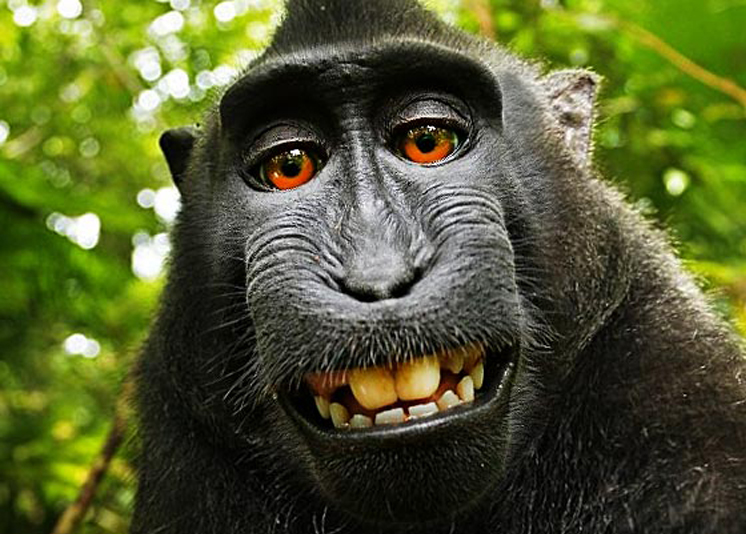
\includegraphics[width=0.5\textwidth]{./figures/selfie_monkey.jpg}
	\caption[Monkey selfie]{This picture is not copyrighted}
	\label{fig:selfie1}
	\end{center}
\end{figure}

Blandit incorrupte quaerendum in quo, nibh impedit id vis, vel no nullam semper audiam. Ei populo graeci consulatu mei, has ea stet modus phaedrum. Inani oblique ne has, duo et veritus detraxit. Tota ludus oratio ea mel, offendit persequeris ei vim. Eos dicat oratio partem ut, id cum ignota senserit intellegat. Sit inani ubique graecis ad, quando graecis liberavisse et cum, dicit option eruditi at duo. Homero salutatus suscipiantur eum id, tamquam voluptaria expetendis ad sed, nobis feugiat similique usu ex.

And now, Table \ref{tab:apvalues} shows some parameter for the Aliev-Panfilov model.
\begin{table}[H]
	\begin{center}
	\caption[Parameters Aliev-Panfilov]{Parameter values considered for the Aliev-Panfilov model of ionic current{\color{red}.}}
	\begin{tabular}{@{}c  c  c  c  c  c  c@{}}\toprule
	$\alpha$	&	$c_1$	&	$c_2$	&	$\mu_{1}$		&	$\mu_2$		&	$b$	&	$\gamma$\\ \midrule
	0.05	&	52	&	8	&	0.1	&	0.3	&	0.25	&	0.002 \\ \bottomrule
	\end{tabular}
	\label{tab:apvalues}
	\end{center}
\end{table}

There are 12 figures in order to show that the List of Figures works fine.

\section{Equations \label{sec:eq}}
Finally, an equation
\begin{equation}
x^2 + 1 = 0
\label{eq:basiceq}
\end{equation}

We can notice that $x=\pm i$ are the solutions of Equation \eqref{eq:basiceq}.

\chapter[CONCLUSIONS]{Conclusions}
Nothing to say. Be happy.

%%%%%%%%%%%%%
%       REFERENCES        %
%%%%%%%%%%%%%

\cleardoublepage
\phantomsection \label{references}
\bibliographystyle{apacite}
\renewcommand{\bibname}{REFERENCES}

%%%% ACTIVAR SIGUIENTES 3 LINEAS SI POSTGRADO RECHAZA LA BIBLIOGRAFIA
%\setlength{\bibleftmargin}{0em}
%\setlength{\bibindent}{0em}
%\setlength{\bibitemsep}{1em}


\bibliography{Thesis}

%%%%%%%%%%%%
%      APPENDICES      %
%%%%%%%%%%%%

\appendix % It is like a chapter, so each appendix (A, B, C...) must to be considered as a section

\newpage
\section[First Appendix]{First Appendix}
We can write equations here too:

\begin{equation}
\int_0^\infty e^{-x^2} dx
\end{equation}

And more...

\newpage
\section[An Interesting Short Story]{An Interesting Short Story}
Let us enjoy reading this story of Hunting With The Lion. 

It was a dry summer. The animals in the forest were beginning to find it difficult to get food. 

A bear, a wolf and a jackal thought it would be better to join hands with a lion and do the hunting. They approached lion and he too agreed. The four of them went off hunting. 

The hunting party came across a buffalo. The fox and wolf chased the buffalo. The bear intercepted the buffalo. The lion killed him. 

The fox made shares out of the buffalo. When they were about to take their shares the lion roared and said, "Well friends, the first share is mine for my leadership. The second share is mine for, it is I who killed. The third share is also mine for I need it for my cubs. Anyone who needs a share can take the fourth. But before that you will have to win me.” 

All the three left the place without a single word. 

MORAL : {\bf If you are might, you are right}.

\end{document}
